\documentclass[1,exos,b,prof,e]{phBook}
%\documentclass[../coursseconde]{subfiles}
%Options : 2, 1, T, SNT (classes), p, b,prof, exos, cours, DS, noir, a4, a5, twocolumn, landscape
%\def\datedevoir{\today} % date du DS à indiquer

\graphicspath{{figures_exercices/}{figures_variations/}}

\begin{document}
\setcounter{chapter}{2} %Numéro du chapitre précédent
\chapter{Exercices : dérivation} %Titre du chapitre
%%%%%%%%%%%%%%%%%%%%%%%%

\footnotesize % petite police

% \begin{exercice}
%     Déterminer, à partir de la définition du nombre dérivé, les nombres dérivés suivants :
%     \begin{enumerate}
%     \item $f'(4)$ pour $f(x)=3x+1$
%     \item $f'(x)$ pour $f(x)=2x-1$
%     \item $f'(2)$ pour $f(x)=4x^2-1$
%     \item $f'(x)$ pour $f(x)=2x^2+3$
%     \end{enumerate}
% \end{exercice}


\qrc{Animation GeoGebra sur le nombre dérivé}{https://phlered.github.io/depot_github/1S/3_Derivation/nb_derive.html}


\begin{exercice}
		$f$ est définie sur $\R$ par $f(x)=2x-5$. 
		\begin{enumerate}
			\item Calculer le taux de variation de $f$ entre $3$ et $3+h$.
			\item En déduire que $f$ est dérivable en $3$ et donner $f'(3)$.
			\item \emph{(Bonus)} Donner $f'(a)$ pour $a$ quelconque.
		\end{enumerate}

		\solution{
			\begin{enumerate}
				\item Le taux de variation de $f$ entre $3$ et $3+h$ est :
				\begin{align*}
				\frac{f(3+h)-f(3)}{h}&=\frac{2(3+h)-5-(2 \cdot 3-5)}{h}\\
				&=\frac{6+2h-5-6+5}{h}\\
				&=\frac{2h}{h}\\
				&=2
				\end{align*}
				\item Donc $f'(3) = 2$.
				\item Pour $a$ quelconque, $f'(a) = 2$.	
			\end{enumerate}
		}
	\end{exercice}








\begin{exercice}
	$f$ est la fonction définie sur $\R$ par :
	\[f(x)=3x^2+1\]
	\begin{enumerate}
		\item Calculer le taux de variation de $f$ entre $4$ et $4+h$.
		\item En déduire que $f$ est dérivable en $4$ et donner $f'(4)$.
	\end{enumerate}

	\solution{
		\begin{enumerate}
			\item
			\begin{align*}
			\frac{f(4+h)-f(4)}{h}
			&=\frac{3(4+h)^2+1-49}{h}\\
			&=\frac{3\left(16+8h+h^2\right)-48}{h}\\
			&=\frac{48+24h+3h^2-48}{h}\\
			&=\frac{24h+3h^2}{h}\\
			&=24+3h
			\end{align*}
			\item Quand $h$ tend vers $0$, $24+3h$ tend vers $24$.
			Donc $f$ est dérivable en $4$ et $f'(4)=24$.
		\end{enumerate}
	}


\end{exercice}


\begin{exercice}
    $f$ est la fonction définie sur $\R^*$ par :
    \[f(x)=\frac{4}{x}\]
    \begin{enumerate}
        \item  Vérifier que pour tout nombre réel $h\in ]-1;0[$ :
        \[\frac{f(1+h)-f(1)}{h}=\frac{-4}{1+h}\]    
        \item En déduire que $f$ est dérivable en $1$ et donner $f'(1)$.
        \item \emph{(Bonus)} Donner $f'(a)$ pour $a \neq 0$ quelconque.
    \end{enumerate}

	\solution{
		\begin{enumerate}
			\item Pour tout $h\in]-1;0[$ :
			\begin{align*}
			\frac{f(1+h)-f(1)}{h}
			&=\frac{\dfrac{4}{1+h}-4}{h}\\
			&=\frac{\dfrac{4-4(1+h)}{1+h}}{h}\\
			&=\frac{-4h}{h(1+h)}\\
			&=\frac{-4}{1+h}
			\end{align*}
			\item Quand $h$ tend vers $0$, $\dfrac{-4}{1+h}$ tend vers $-4$.
			Donc $f$ est dérivable en $1$ et $f'(1)=-4$.
			\item Pour $a\neq 0$ :
			\begin{align*}
			\frac{f(a+h)-f(a)}{h}
			&=\frac{\dfrac{4}{a+h}-\dfrac{4}{a}}{h}\\
			&=\frac{\dfrac{4a-4(a+h)}{a(a+h)}}{h}\\
			&=\frac{-4h}{h\,a(a+h)}\\
			&=\frac{-4}{a(a+h)}
			\end{align*}
			Quand $h$ tend vers $0$, on obtient $f'(a)=\dfrac{-4}{a^2}$.
		\end{enumerate}
	}


\end{exercice}


\begin{exercice}
    $f$ est la fonction définie sur $\R$ par :
    \[f(x)=2x^2-3x\]
    \begin{enumerate}
        \item  Calculer le taux de variation de $f$ entre $a$ et $a+h$.    
        \item En déduire que $f$ est dérivable en $a$ et donner $f'(a)$.
    \end{enumerate}

	\solution{
		\begin{enumerate}
			\item
			\begin{align*}
			\frac{f(a+h)-f(a)}{h}
			&=\frac{2(a+h)^2-3(a+h)-\left(2a^2-3a\right)}{h}\\
			&=\frac{2a^2+4ah+2h^2-3a-3h-2a^2+3a}{h}\\
			&=\frac{4ah+2h^2-3h}{h}\\
			&=4a+2h-3
			\end{align*}
			\item Quand $h$ tend vers $0$, $4a+2h-3$ tend vers $4a-3$.
			Donc $f$ est dérivable en $a$ et $f'(a)=4a-3$.
		\end{enumerate}
	}


\end{exercice}





% \begin{exercice} On a représenté la courbe d'une fonction $f$. Les points $A$, $B$, $C$ et $D$ sont des points de la courbe de $f$  d'abscisses respectives $0$, $1$, $2$ et $-1$.
%     % \begin{definition*}
%     % On appelle tangente au point $A$ d'abscisse $a$ à la courbe $C_{f}$ la droite passant
%     % par $A$ de coefficient directeur $f'\left(a\right)$.\end{definition*}
%      Les droites en pointillé représentent les tangentes en ces points à la courbe de $f$. 
%     \begin{center}
%     \includegraphics[width=1\columnwidth]{chercher_les_nombres_derivees}
%     \end{center}
    
%     % \begin{enumerate}
%     % \item 
%     Compléter le tableau ci-dessous :
    
%     \begin{center}
%     \begin{tabular}{|c|c|c|c|c|}
%     \hline 
%     point & $A$ & $B$ & $C$  & $D$\tabularnewline
%     \hline 
%     valeur de $x$ &  &  &  & \tabularnewline
%     \hline 
%     $f'\left(x\right)$ &  &  &  & \tabularnewline
%     \hline 
%     \end{tabular}
%     \end{center}
%     % \item On donne : $f\left(x\right)=x^{3}-2$. Déterminer $f'\left(x\right)$ et vérifier les valeurs précédentes.
%     % \end{enumerate}
% \end{exercice}
    



    
\begin{exercice}
 \noindent

% 	\begin{tikzpicture}[>=stealth, scale=0.8]

% %---- Grille ----%
% \draw[step=0.5cm, gray!40, very thin] (-7,-4) grid (7,8);
% \draw[step=1cm, gray!70, thin] (-7,-4) grid (7,8);

% %---- Axes ----%
% \draw[thick, ->] (-7,0) -- (7,0) node[right] {$x$};
% \draw[thick, ->] (0,-4) -- (0,8) node[above] {$y$};

% %---- Parabole C ----%
% \draw[blue, thick, domain=-6:5, samples=200]
%      plot (\x, 0.5*(\x+2)^2 - 2) node[pos=0.05, left, blue] {$\mathcal C$};

% %---- Tangente noire ----%
% % droite passant par (0,0) et (3,6)
% \draw[thick]
%       (-1,-2) -- (6,8);

% % Point B
% \fill (3,6) circle (2pt);
% \node[right] at (3,6) {$B$};

% %---- Tangente bleue ----%
% \draw[blue, very thick]
%       (-6,7) -- (4.5,7); % segment supérieur (pour visuel conforme)

% % Petit segment inclinée (sur la parabole)
% \draw[blue, thick]
%       (-2.5,-1.5) -- (2,2.5);

% %---- Petite droite passant par l’origine (D) ----%
% \draw[thick] (-2,-3) -- (1.5,1);
% \node at (-1.2,-2.5) {$D$};

% \end{tikzpicture}


\begin{minipage}{0.35\linewidth}
	    Soit $f$ la fonction définie sur l’intervalle $[-6 ; 4]$ et dont la courbe $\mathcal{C}$ est représentée ci-contre.
    On admet que la fonction $f$ est dérivable sur l’intervalle  $[-6 ; 4]$.

    La tangente au point d'abscisse $0$ passe par le point $B$.

	    \begin{enumerate}
        \item Déterminer $f'(0)$
        % \item Résoudre à partir du graphique l'équation $f(x)=0$
        \item Résoudre l'équation $f'(x)=0$ (Expliquer)
    \end{enumerate}
    

\end{minipage}
\hfill
\begin{minipage}{0.6\linewidth}
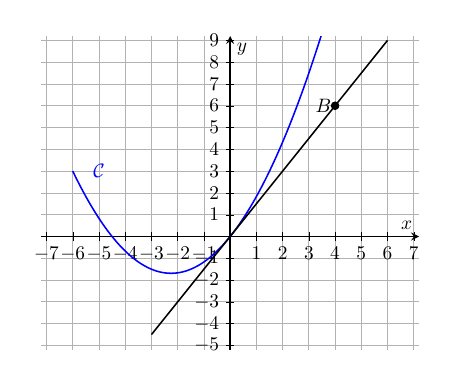
\begin{tikzpicture}[scale=0.70]
\begin{axis}[
	axis lines=middle,
	xlabel={$x$},
	ylabel={$y$},
	xmin=-6, xmax=6,
	ymin=-4, ymax=8,
	grid=both,
	grid style={gray!30},
	major grid style={gray!60},
	axis line style={thick},
	tick style={black},
	xtick distance=1,
	ytick distance=1,
	% width=14cm, height=10cm,
	enlargelimits=true,
]


% -------- Parabole C --------
\addplot [
    domain=-6:5,
    samples=200,
    thick,
    blue
] {1/3*x^2+1.5*x};
\node[blue] at (axis cs:-5,3) {$\mathcal C$};

% -------- Tangente noire (O vers B) --------
\addplot [
    thick,
    black
] coordinates {(-3,-4.5) (6,9)	};

% Point B
\addplot[only marks, mark=*] coordinates {(4,6)};
\node[right] at (axis cs:3,6) {$B$};

\end{axis}
\end{tikzpicture}

\end{minipage}

	\solution{
		\begin{enumerate}
			\item La tangente au point d'abscisse $0$ passe par $O(0;0)$ et par $B(4;6)$,
			donc son coefficient directeur est
			\[f'(0)=\frac{6-0}{4-0}=\frac{3}{2}=1,5.\]
			\item $f'(x)=0$ lorsque la tangente à la courbe est horizontale, c'est-à-dire
			au sommet de la parabole. Graphiquement, ce point a pour abscisse $x\approx-2$.
			Donc l'équation $f'(x)=0$ a pour solution $x=-\dfrac{9}{4}$.
		\end{enumerate}
	}


\end{exercice}




\begin{exercice}
    La fonction $f$ est représentée ci-dessous
    ainsi que ses tangentes aux points d'abscisses $-2$, $-1$, $0$,
    1 et 2.
    \begin{center}
    \includegraphics[width=0.9\linewidth]{Capture_tangentes}
    \end{center}
    \begin{enumerate}
        \item Déterminer graphiquement $f'\left(-2\right)$, $f'\left(-1\right),$
        $f'\left(0\right),$ $f'\left(1\right),$ $f'\left(2\right)$.
        \item On donne :  $f\;:\ x\mapsto\frac{1}{2}x^{2}-x$.
        Déterminer, pour tout réel $x$, $f'(x)$, puis retrouver par le calcul les valeurs précédentes.
    \end{enumerate}

	\solution{
		\begin{enumerate}
			\item On lit le coefficient directeur de chaque tangente tracée :
			\[f'(-2)=-3,\quad f'(-1)=-2,\quad f'(0)=-1,\]
			\[f'(1)=0,\quad f'(2)=1.\]
			\item Pour tout réel $x$, $f'(x)=\frac{1}{2}\times 2x-1=x-1$.
			On retrouve bien les valeurs lues sur le graphique.
		\end{enumerate}
	}


\end{exercice}
    

% \begin{exercice}
% Déterminer, à partir de la définition du nombre dérivé, les nombres dérivés suivants :
% \begin{enumerate}
% \item $f'(4)$ pour $f(x)=3x+1$
% \item $f'(x)$ pour $f(x)=2x-1$
% \item $f'(2)$ pour $f(x)=4x^2-1$
% \item $f'(x)$ pour $f(x)=2x^2+3$
% \end{enumerate}
% \end{exercice}
%\begin{exercice}
%Déterminer la dérivée des fonctions suivantes :
%\begin{enumerate}
%\item $f(x)=-3x^2+8x-2$  sur $\mathbb{R}$ ;
%\item $f(x)=2x^3-4x^2+5x+1$  sur $\mathbb{R}$ ;
%\item $f(x)=\frac{5}{x}$ pour $x\neq 0$ ;
%\item $f(x)=(x^2+x+x)(2x-5)$ sur $\mathbb{R}$ ;
%\item $f\left(x\right)=\left(3x+1\right)\sqrt{x}$ pour $x>0$ ;
%
%%\item $f\left(x\right)=\frac{2x-1}{3x+9}$ pour $x\neq-3$.
%%\item $f\left(x\right)=\left(2x^{2}-3x+1\right)^{2}$ sur $\mathbb{R}$ ;
%\end{enumerate}
%\end{exercice}



% \begin{activite}
%     Notons $C_{f}$ la courbe dans un repère d'une fonction $f$ définie
%     sur un intervalle $I$. Soit $a\in I$ et $A$ un point de la courbe
%     d'abscisse $a$.
%     %\begin{definition*}
%     %On appelle tangente en $A$ à la courbe $C_{f}$ la droite passant
%     %par $A$ de coefficient directeur $f'\left(a\right)$.\end{definition*}
%     \begin{enumerate}
%     \item Quelles sont les coordonnées de $A$ ?
%     \item Démontrer qu'une équation de la tangente en $A$ à la courbe est :
%     \[y=f'\left(a\right)\left(x-a\right)+f\left(a\right)\]
%     \item Exemple 1 : $f\left(x\right)=x^{2}$, $A$ le point de $C_{f}$ d'abscisse
%     $3$. Donner une équation de la tangente en $A$ à la courbe de $f$.
%     \item Exemple 2 : $f\left(x\right)=\frac{1}{x}$, $A$ le point de $C_{f}$
%     d'abscisse $2$. Donner une équation de la tangente en $A$ à la courbe
%     de $f$.
%     \end{enumerate}
% \end{activite}





% \begin{exercice}
% En utilisant le formulaire, déterminer les nombres dérivés suivants :
% \begin{enumerate}
% \item $f'(1)$ pour $f(x)=3$
% \item $f'(3)$ pour $f(x)=2x-5$
% \item $f'(5)$ pour $f(x)=x^2$
% \item $f'(0,5)$ pour $f(x)=\frac{1}{x}$
% \end{enumerate}
% \end{exercice}



% \begin{exercice}
% A partir du formulaire, retrouver les nombres dérivés pour les questions 3.  et 4. de l'exercice 1
% \end{exercice}




\begin{exercice}
	Déterminer la fonction dérivée pour chacune des fonctions suivantes :
	\begin{enumerate}
		\item $f(x)=5x^2-3x+2$ définie sur $\R$
		\item $f(x)=x^3-4x^2+3x+5$ définie sur $\R$
		\item $f(x)=\frac{1}{3}x^3+\frac{1}{2}x^2+x+1$ définie sur $\R$
		\item $f(x)=\frac{4}{x}$ définie sur $]0;+\infty[$
	\end{enumerate}

	\solution{
		\begin{enumerate}
			\item $f'(x)=10x-3$
			\item $f'(x)=3x^2-8x+3$
			\item $f'(x)=x^2+x+1$
			\item $f'(x)=-\frac{4}{x^2}$
		\end{enumerate}
	}


\end{exercice}





\begin{exercice}
	Déterminer la dérivée des fonctions suivantes :
	\begin{enumerate}
		\item $f(x)=5 x^2-3 x+2$ définie sur $\mathbb{R}$
		\item $f(x)= 100+\frac{1}{x}$ définie sur $\mathbb{R}^*$
		\item $f(x)= x \sqrt{x}$ définie sur $[0 ;+\infty[$
		\item $f\left(x\right)=\frac{1}{2x-4}$ sur $]2;+\infty[$
		\item $f(x)=\frac{-3}{x^2-4}$ sur $]-2;2[$ ;
		\item $f\left(x\right)=\frac{2x-1}{3x+9}$ pour $x\neq-3$ ;
		\item $f(x)=\frac{5x+1}{2x-4}$ pour $x\neq 2$ ;
		% \item $f(x)=\frac{3x+2}{2x+6}$ pour $x\neq -3$
		\item $f\left(x\right)=\left(2x^{2}-3x+1\right)^{2}$ sur $\mathbb{R}$.
	\end{enumerate}

	\solution{
		\begin{enumerate}
			\item $f'(x)=10x-3$
			\item $f'(x)=-\frac{1}{x^2}$
			\item $f'(x)=\sqrt{x}+x\times\frac{1}{2\sqrt{x}}
			=\sqrt{x}+\frac{\sqrt{x}}{2}=\frac{3\sqrt{x}}{2}$ \ (pour $x>0$)
			\item $f'(x)=\frac{-2}{(2x-4)^2}$
			\item $f'(x)=\frac{6x}{(x^2-4)^2}$
			\item $f'(x)=\frac{21}{(3x+9)^2}=\frac{7}{3(x+3)^2}$
			\item $f'(x)=\frac{-22}{(2x-4)^2}=\frac{-11}{2(x-2)^2}$
			\item $f'(x)=2\left(2x^2-3x+1\right)(4x-3)$
		\end{enumerate}
	}


\end{exercice}





\begin{exercice}
    On considère la fonction $f$ définie sur $\mathbb{R}$ par 
    \[f\left(x\right)=3x^{2}-2x+2\]
    %La courbe de $f$ admet-elle une tangente passant par $A\left(1;-1\right)$?
    Déterminer une équation de la tangente à la courbe de $f$ au point d'abscisse $2$.

	\solution{
		$f'(x)=6x-2$, donc $f'(2)=10$, et $f(2)=3\times 4-4+2=10$.
		Une équation de la tangente au point d'abscisse $2$ est
		\[y=f'(2)(x-2)+f(2)=10(x-2)+10=10x-10.\]
	}


\end{exercice}
    



\begin{exercice}
Soit $f\left(x\right)=$$\frac{3x+4}{2x+4}$ pour $x\neq-2$.
\begin{enumerate}
\item Déterminer $f'\left(x\right)$
\item En quels points de la courbe de $f$ y a t-il une tangente parallèle
à la droite d'équation $y=x$ ?
\end{enumerate}

	\solution{
		\begin{enumerate}
			\item Pour $x\neq-2$ :
			\[f'(x)=\frac{3(2x+4)-2(3x+4)}{(2x+4)^2}
			=\frac{4}{(2x+4)^2}=\frac{1}{(x+2)^2}.\]
			\item La tangente est parallèle à la droite d'équation $y=x$ si et seulement
			si $f'(x)=1$ :
			\[\frac{1}{(x+2)^2}=1 \iff (x+2)^2=1 \iff x=-1 \text{ ou } x=-3.\]
			Les points cherchés sont donc
			$A\left(-1;\frac{1}{2}\right)$ et $B\left(-3;\frac{5}{2}\right)$.
		\end{enumerate}
	}


\end{exercice}
        
    
    
\begin{exercice}
    On considère la fonction $f$ définie sur $\mathbb{R}$ par $f\left(x\right)=-x^{2}+3x$,
    on note $\mathcal{C}_{f}$ sa courbe représentative.
    \begin{center}
    \includegraphics[width=0.7\linewidth]{tangente_parabole_eleve}
    \end{center}
    \begin{enumerate}
    \item Déterminer une équation de la tangente à la courbe au point d'abscisse
    $1$.
    \item Le point $A$ a pour coordonnées $\left(4;0\right)$. Déterminer les
    tangentes à $\mathcal{C}_{f}$ passant par $A$.
    \item Même question avec le point $B\left(2;3\right)$.
    \end{enumerate}

	\solution{
		\begin{enumerate}
			\item $f'(x)=-2x+3$, donc $f'(1)=1$ et $f(1)=2$.
			La tangente au point d'abscisse $1$ a pour équation
			$y=1(x-1)+2=x+1$.
			\item Une tangente au point d'abscisse $a$ a pour équation
			\[y=(-2a+3)(x-a)-a^2+3a.\]
			Elle passe par $A(4;0)$ si et seulement si
			\begin{align*}
			0&=(-2a+3)(4-a)-a^2+3a\\
			&=2a^2-11a+12-a^2+3a\\
			&=a^2-8a+12=(a-2)(a-6).
			\end{align*}
			Donc $a=2$ ou $a=6$, et les tangentes cherchées sont
			$y=-x+4$ et $y=-9x+36$.
			\item Elle passe par $B(2;3)$ si et seulement si
			\begin{align*}
			3&=(-2a+3)(2-a)-a^2+3a\\
			&=2a^2-7a+6-a^2+3a\\
			&=a^2-4a+6
			\end{align*}
			donc $a^2-4a+3=0$, soit $(a-1)(a-3)=0$.
			Les tangentes cherchées sont $y=x+1$ et $y=-3x+9$.
		\end{enumerate}
	}


\end{exercice}
    
    
\begin{exercice}
	$f$ est une fonction définie sur $\R$ par
	$f(x)=a x^2+b x+c$ où $a, b$ et $c$ sont des réels.
	$C_f$ est sa courbe représentative dans un repère $\left(O;I,J\right)$.
	On sait que $C _f$ passe par l'origine du repère et que la droite d'équation $y=3 x-5$ est tangente à $C _f$ au point $A$ d'abscisse $-2$.
	\begin{enumerate}
		\item Déterminer le réel $c$.
		\item Déterminer les coordonnées du point $A$.
		\item En déduire les réels $a$ et $b$.
	\end{enumerate}
	\solution[0]{
		\begin{enumerate}
			\item $f(0)=0 \Leftrightarrow c=0$
			\item Le point A est sur la tangente alors :
			\[
			y_A=3 \times (-2) - 5 = 1 \text{. Donc } A(-2; 1).
			\]
			\item On sait que $A \in C_f$ alors $f(-2)=1$, c'est-à-dire $4a - 2b = 1$.
			D'autre part, $f'(-2)=3$ car le coefficient directeur de la tangente en $A$ est égal à 3. Or, pour tout réel $x$, $f'(x)=2ax + b$. Donc, on a $-4a + b = 3$.
			En résolvant le système 
			\[
			\begin{cases}
			4a - 2b = 1 \\
			-4a + b = 3
			\end{cases}
			\]
			on trouve $b = -4$ et $a = -\frac{7}{4}$.
		\end{enumerate}
	}
\end{exercice}

\begin{exercice}
	On considère la fonction $f$ définie sur $]0;+\infty[$ par $f(x)=\sqrt{x}$.
	\begin{enumerate}
		\item Calculer $f'(x)$ puis $f'(1)$.
		\item Pour $h$ proche de $0$, on utilise l'approximation linéaire
		$f(1+h)\approx f(1)+f'(1)h$. En déduire une valeur approchée de $\sqrt{1,02}$.
		\item Vérifier à la calculatrice. L'approximation est-elle satisfaisante ?
		\item \emph{(Bonus)} La fonction $g$ est définie sur $\R^*$ par $g(x)=\dfrac{1}{x}$.
		Donner de même une valeur approchée de $\dfrac{1}{1,01}$.
	\end{enumerate}

	\solution{
		\begin{enumerate}
			\item $f'(x)=\dfrac{1}{2\sqrt{x}}$, donc $f'(1)=\dfrac{1}{2}$.
			\item $\sqrt{1,02}=\sqrt{1+0,02}\approx f(1)+f'(1)\times 0,02
			=1+\dfrac{1}{2}\times 0,02=1,01$.
			\item La calculatrice donne $\sqrt{1,02}\approx 1,00995$.
			L'erreur est inférieure à $10^{-4}$ : l'approximation est très bonne.
			\item $g'(x)=-\dfrac{1}{x^2}$, donc $g'(1)=-1$ et
			$\dfrac{1}{1,01}\approx g(1)+g'(1)\times 0,01=1-0,01=0,99$
			(la calculatrice donne $0,990099\ldots$).
		\end{enumerate}
	}
\end{exercice}


\begin{exercice}
	\begin{enumerate}
		\item La fonction $f$ est définie sur $\R$ par $f(x)=|x|$.
		\begin{enumerate}
			\item Calculer $\dfrac{f(0+h)-f(0)}{h}$ pour $h>0$, puis pour $h<0$.
			\item Que peut-on en déduire pour la dérivabilité de $f$ en $0$ ?
			Interpréter graphiquement.
		\end{enumerate}
		\item La fonction $g$ est définie sur $[0;+\infty[$ par $g(x)=\sqrt{x}$.
		Montrer que, pour tout $h>0$, $\dfrac{g(h)-g(0)}{h}=\dfrac{1}{\sqrt{h}}$,
		puis en déduire que $g$ n'est pas dérivable en $0$.
	\end{enumerate}

	\solution{
		\begin{enumerate}
			\item
			\begin{enumerate}
				\item Pour $h>0$, $f(h)=h$ donc
				$\dfrac{f(0+h)-f(0)}{h}=\dfrac{h}{h}=1$.
				Pour $h<0$, $f(h)=-h$ donc
				$\dfrac{f(0+h)-f(0)}{h}=\dfrac{-h}{h}=-1$.
				\item Le taux de variation ne tend pas vers la même valeur à droite
				($1$) et à gauche ($-1$) de $0$ : $f$ n'est donc pas dérivable en $0$.
				Graphiquement, la courbe présente un « angle » en $O$ : il n'y a pas
				de tangente unique en $0$.
			\end{enumerate}
			\item Pour $h>0$ :
			$\dfrac{g(h)-g(0)}{h}=\dfrac{\sqrt{h}}{h}=\dfrac{1}{\sqrt{h}}$.
			Or $\dfrac{1}{\sqrt{h}}$ devient aussi grand que l'on veut lorsque $h$
			tend vers $0$ : le taux de variation n'admet pas de limite finie.
			Donc $g$ n'est pas dérivable en $0$ (la tangente en $O$ serait verticale).
		\end{enumerate}
	}
\end{exercice}



\begin{exercice}
	On considère la fonction $f$ définie sur $\R$ par $f(x)=x^2$ et $\mathcal{C}$
	sa courbe représentative.
	\begin{enumerate}
		\item Déterminer une équation de la tangente $T$ à $\mathcal{C}$ au point
		d'abscisse $1$.
		\item Montrer que, pour tout réel $x$, $f(x)-(2x-1)=(x-1)^2$.
		\item En déduire la position relative de $\mathcal{C}$ et de $T$. Pour quelle
		valeur de $x$ les deux courbes se coupent-elles ?
	\end{enumerate}

	\solution{
		\begin{enumerate}
			\item $f'(x)=2x$, donc $f'(1)=2$, et $f(1)=1$. La tangente en $1$ a pour
			équation $y=2(x-1)+1=2x-1$.
			\item $f(x)-(2x-1)=x^2-2x+1=(x-1)^2$.
			\item Un carré est toujours positif ou nul, et $(x-1)^2=0$ seulement pour
			$x=1$. Donc $\mathcal{C}$ est toujours au-dessus de $T$, et les deux
			courbes n'ont qu'un seul point commun : le point de contact $(1;1)$.
		\end{enumerate}
	}
\end{exercice}




% \begin{exercice} On a représenté la courbe d'une fonction $f$. Les points $A$, $B$, $C$ et $D$ sont des points de la courbe de $f$  d'abscisses respectives $0$, $1$, $2$ et $-1$.
% \begin{definition*}
% On appelle tangente au point $A$ d'abscisse $a$ à la courbe $C_{f}$ la droite passant
% par $A$ de coefficient directeur $f'\left(a\right)$.\end{definition*}
%  Les droites en pointillé représentent les tangentes en ces points à la courbe de $f$. 
% \begin{center}
% \includegraphics[width=1\columnwidth]{chercher_les_nombres_derivees}
% \end{center}

% \begin{enumerate}
% \item Compléter le tableau ci-dessous :

% \begin{center}
% \begin{tabular}{|c|c|c|c|c|}
% \hline 
% point & $A$ & $B$ & $C$  & $D$\tabularnewline
% \hline 
% valeur de $x$ &  &  &  & \tabularnewline
% \hline 
% $f'\left(x\right)$ &  &  &  & \tabularnewline
% \hline 
% \end{tabular}
% \end{center}
% \item On donne : $f\left(x\right)=x^{3}-2$. Déterminer $f'\left(x\right)$ et vérifier les valeurs précédentes.
% \end{enumerate}
% \end{exercice}




%\begin{exercice}
%La fonction $f$ est représentée ci-dessous
%ainsi que ses tangentes aux points d'abscisses $-2$, $-1$; $0$;
%1 ; 2.
%\begin{center}
%\includegraphics[width=\columnwidth]{Capture_tangentes}
%\end{center}
%\begin{enumerate}
%\item Déterminer graphiquement $f'\left(-2\right)$, $f'\left(-1\right),$
%$f'\left(0\right),$ $f'\left(1\right),$ $f'\left(2\right)$.
%\item On donne :  $f\;:\ x\mapsto\frac{1}{2}x^{2}-x$. Déterminer, pour tout réel $x$, $f'(x)$, puis retrouver par le calcul les valeurs précédentes.
%\end{enumerate}
%\end{exercice}
%








%\begin{exercice}
%Soient $\mathcal{C}_{f}$ et $\mathcal{C}_{g}$ les courbes représentatives
%des fonctions $f$ et $g$ définies sur $\mathbb{R}$ par $f\left(x\right)=x^{2}$
%et $g\left(x\right)=x^{2}+2x+3$. $A$ est point de $\mathcal{C}_{f}$
%d'abscisse $a$ et $B$ est un point de $\mathcal{C}_{g}$ d'abscisse
%$b$.
%\begin{enumerate}
%\item Déterminer une équation des tangentes en $A$ et $B$ aux courbes
%de $f$ et $g$.
%\item Démontrer que $\left(AB\right)$ est une tangente commune à $\mathcal{C}_{f}$
%et $\mathcal{C}_{g}$si et seulement si
%\[\begin{cases}
%a & =b+1\\
%a^{2} & =b^{2}-3
%\end{cases}\]
%\item En déduire les coordonnées de $A$ et de $B$ pour que $\mathcal{C}_{f}$
%et $\mathcal{C}_{g}$ aient une tangente commune.\end{enumerate}
%\end{exercice}






% % DM ???
% \begin{exercice}
% La trajectoire d'un avion est portée par la courbe $\mathcal{C}$ d'équation
% $y=\frac{1}{x}$ dans un repère orthonormé. On admet que lorsqu'il
% lâche une bombe au point $M$, la bombe poursuit son mouvement en
% ligne droite sur la tangente en $M$. A quel endroit doit-il lâcher
% sa bombe pour qu'elle atteigne le point $A\left(4;0\right)$ ?
% \end{exercice}







% % DM ????
% \begin{exercice}
%     Dans un repère orthonormal, $\mathcal{P}$ est la parabole d'équation
%     $y=x^{2}$ et $\mathcal{D}$ est la droite d'équation $y=2x+3$. La
%     droite $\mathcal{D}$ coupe $\mathcal{P}$ en $A$ et $B$. On note
%     $I$ le milieu de $\left[AB\right]$.
%     \begin{enumerate}
%         \item Calculer les coordonnées des points $A$ et $B$, puis les coordonnées
%         de $I$.
%         \item Déterminer le point $H$ de $\mathcal{P}$ en lequel la tangente est
%         parallèle à $\left(AB\right)$.
%         \item Que peut-on dire des points $I$ et $H$ ? 
%     \end{enumerate}
% \end{exercice}



















%\begin{exercice}
%Dans un repère, $\mathcal{P}$ et $\mathcal{H}$ sont les courbes
%représentatives des fonctions $f\left(x\right)=x^{2}$ et $g\left(x\right)=\frac{1}{x}\quad(x\neq0)$.
%$\mathcal{P}$ et $\mathcal{H}$ ont-elles une tangente commune ?
%(c'est à dire une droite tangente en $A$ à $\mathcal{P}$ et en $B$ à $\mathcal{H})$
%\end{exercice}
%





%\begin{exercice}
%\begin{enumerate}
%\item Démontrer que $\sqrt{3}-\sqrt{2}=\frac{1}{\left(\sqrt{3}+\sqrt{2}\right)}$.
%Plus généralement, exprimer $\sqrt{b}-\sqrt{a}$ en fonction de $\sqrt{b}+\sqrt{a}$.
%\item A partir de la définition du nombre dérivé, démontrer que $\left(\sqrt{x}\right)'=\frac{2}{\sqrt{x}}$
%\item Déterminer une équation de la tangente à la courbe représentant $x\mapsto\sqrt{x}$
%au point d'abscisse $4$.\end{enumerate}
%\end{exercice}

% on pourra rafraîchir les connaissances avec les activités 1 à 5 page 88



% \begin{activite}
% Ci-dessous est tracée la courbe représentative d'une fonction $f$.
% En pointillés sont tracées quelques tangentes.
% \begin{center}
% \includegraphics[width=\linewidth]{activite_intro_eleves}
% \end{center}
% \begin{enumerate}
% \item A partir du graphique, compléter le tableau suivant :
% \begin{center}
% \begin{tabular}{|c|c|c|c|c|c|c|c|c|}
% \hline 
% $x$ & $-2$ & $-1$ & $0$ & $1$ & $2$ & $3$ & $4$ & $5$\tabularnewline
% \hline 
% \hline 
% Signe de $f'\left(x\right)$ &  &  &  &  &  &  &  & \tabularnewline
% \hline 
% \end{tabular}
% \end{center}
% \item Que pouvez-vous conjecturer sur le signe de $f'\left(x\right)$ ?
% \item Donner le tableau de variations de $f$.
% \item Qu'observez-vous ?
% \end{enumerate}
% \end{activite}





% \begin{activite}
% \begin{enumerate}
% \item 
% On considère une fonction $f$ croissante sur un intervalle $I$. Soit $x\in I$.
% \begin{enumerate}
% \item Quel est le signe de $f\left(x+h\right)-f\left(x\right)$ quand $h>0$
% ? Quel est alors le signe de $\frac{f\left(x+h\right)-f\left(x\right)}{h}$
% ?
% \item Quel est le signe de $\frac{f\left(x+h\right)-f\left(x\right)}{h}$
% quand $h<0$ ?
% \item En déduire le signe de $f'\left(x\right)$.
% \end{enumerate}
% \item Quel est le signe de $f'\left(x\right)$ quand $f$ est décroissante
% sur $I$ ?
% \item Qu'avez-vous démontré ?
% \end{enumerate}
% \end{activite}





%%%%%%%%%%%%%%%%%%% EXERCICES %%%%%%%%%%%%%



% \begin{exercice}
% %[sens de variation d'une fonction trinôme : étude d'un cas particulier]
% On considère la fonction $f$ définie sur $\R$ par $$f(x)=-x^2+6x-1$$
% \begin{enumerate}
% \item A l'aide de vos connaissances sur les fonctions trinômes (deuxième chapitre), déterminer le sens de variation de $f$.
% \item 
% 	\begin{enumerate}
% 	\item Déterminer $f'\left(x\right)$
% 	\item Étudier le signe de $f'\left(x\right)$.
% 	\item Retrouvez le résultat de la première question
% 	\end{enumerate}
% \end{enumerate}
% \end{exercice}






% \begin{exercice}[sens de variation d'une fonction trinôme : cas général]
% On considère $f$ définie par $f\left(x\right)=ax^{2}+bx+c$
% \begin{enumerate}
% \item Rappeler, suivant le signe de $a$, le sens de variations de $f$.
% \item 
% 	\begin{enumerate}
% 	\item Déterminer $f'\left(x\right)$
% 	\item Étudier le signe de $f'\left(x\right)$ si $a>0$ puis si $a<0$.
% 	\item Retrouvez le résultat de la première question
% 	\end{enumerate}
% \end{enumerate}
% \end{exercice}





\end{document}






\end{document}